\documentclass[11pt]{report}

\usepackage{epsf,amsmath,amsfonts}
\usepackage{graphicx}
\usepackage{color}

\setlength{\textwidth}{6.5in}
\setlength{\oddsidemargin}{0in}
\setlength{\evensidemargin}{0in}
\setlength{\textheight}{8.5in}
\setlength{\topmargin}{0in}

\begin{document}

\title{
Requirements and Design\\
Ocean Analysis Core (OAC)}
\author{MPAS Development Team}

\maketitle
\tableofcontents

%-----------------------------------------------------------------------

\chapter{Summary}

Now that MPAS-O is well developed and tested, it is time to add an extensible and forward-looking analysis functionality to the MPAS-Ocean model.  Much of the analysis (diagnostics) developed to date has used a post-processing work-flow with Matlab or Python.  These tools have been useful to meet short-term requirements, but they do not scale well to high resolution, and are typically created individually by each developer without coordination, review, or commits to the repository.

This design document lays out a new ocean analysis functionality, where analysis modules such as global means, zonal means, MOC, Lagrangian particles, etc, may be called at run time from the ocean core or as a post-processing step using the Ocean Analysis Core (OAC).  Advantage are that all MPAS grid variables and operators are available within the analysis modules; analysis routines will fall under the same review process and revision control as other code; and once developed, analysis routines are available to all users.

This document only deals with the overall design of the analysis modules and analysis core, not the details of any new diagnostics added within this new framework.  The global diagnostics, which already exist, will be used to test this new design. 

%-----------------------------------------------------------------------

\chapter{Requirements}

\section{Overall organization}
\subsection{Requirement: OAC may be executed in-situ (i.e. during runtime) or as a post-processing step.}

\subsection{Requirement: When executed in-situ, OAC may be conducted on the same processors as used for the forward model or on a separate set of processor. In that, OAC can execute in single-program, multiple-data (SPMD) or multiple-program, multiple-data (MPMD) mode. \label{requirement: modes}}
Stated otherwise, OAC can be executed ``in-line'' (OAC-SPMD) with the forward model and can be called (when needed) as a part of the time-stepping sequence. Alternatively, OAC can be executed with a separate MPI communicator (OAC-MPMD) and, thus, executed on dedicated processors that are different from those used for the forward model integration.

This requirement will not be part of the initial implementation due to its complexity, but should not be built out of the design.

\subsection{{\color{red} Requirement}: Single or separate executables in MPMD mode}

A requirement yet to be determined is whether OAC-MPMD runs within one or two exectuables.  In the case of two, one would be compiled from the ocean core, the other from the OAC.  Both would be launched simultaniously on separate groups of processors, and they would likely communicate with sockets.  MPMD will not be in the initial implementation, so this decision will be delayed.

\subsection{Requirement: Analysis computations will be organized in groups of related computations, controlled in a coherent manner.}
Each {\it analysis member} will have an identical template structure for namelists and code, including flags, timers, init and finalize routines, and the top-level subroutine interface. A template will be included to guide developers for the creation of a new OAC analysis member.

\subsection{Requirement: Analysis algorithms are unaware of the executing environment.}
Below the OAC driver level, the analysis methods are incognizant of whether the operating environment is OAC-SPMD, OAC-MPMD or OAC-PP.

\subsection{Requirement: Each OAC analysis member is compiled into its own library.}
In order to promote modularity and reuse of object code, each analysis member is to be compiled into its own library that are loaded, along with a driver, to produce OAC.  This will ease the future building of MPMD capability.

\newpage
\section{Input data and files}

\subsection{{\color{red} Requirement}: Variable ownership and modification.}
\begin{itemize}
\item Each AM will ``own'' a set of variables.
\item The AM variable set may only be altered within that AM module.
\item An AM module may not alter any variables other than its own AM variable set (i.e. all other variables are intent(in)).
\end{itemize}
For example, the global\_stats AM will own variables pertaining to global minimum, maximum, and means.  These will be placed in a variable structure for that AM.

\subsection{Requirement: When viewed from the OAC driver and from each OAC analysis member, intent(in) variables are ``state'' and ''analysisInput'' derived data types. Our aspiration is that ``analysisInput'' is empty.}
The modularity, extensibility and repurposing of OAC analysis member will be optimized by limiting the scope of intent(in). The optimal realization of this aspiration would be that OAC operates with only knowledge of the MPAS-O prognostic variables. The requirement here acknowledges our imperfect knowledge of the feasibility of this aspiration.

The upside benefit of this approach is that by minimizing the data flow between MPAS-O and OAC, we reduce risks related to communication bottlenecks and redundant memory allocations. Furthermore, if intent(in) is entirely contained within state, OAC will be able to execute with access of output files or restart files. The downside risk that relatively expensive computations might have to be recomputed. Furthermore, it may turn out that analysis members will require accumulated and/or time-averaged fields from MPAS-O. Thus, we allow for the creation of a new derived data type, {\bf analysisInput}, where auxiliary data can be transferred to OAC. We set a very high bar of adding variable arrays into {\bf analysisInput}.

\newpage
\section{Analysis Member Output}
\subsection{Requirement: Output file format will be netCDF}
All analysis members will write netCDF files along with the derived meta data from the registry in manner identical the current paradigm with MPAS-O. Additional types of output format are permitted, but auxiliary workflow items should be constructed on top of the self-describing netCDF output files. This includes hooks into Paraview, UV-CDAT and similar.

\subsection{{\color{red} Requirement}: Each analysis member will write to a unique output file and may specify its own write frequency.}
This needs to wait for  multiple streams.  Until that time, all OAC data will be written to the standard output*.nc file.


\newpage
\section{Code structure}
\subsection{Requirement: Redundant computations are computed with identical software.\label{requirement: redundant code}}
This means that computation of diagnostic variables like kinetic energy would not appear in both the ocean and analysis cores. The implementation of this requirement is to force a more modular computation of auxiliary (i.e. diagnostic) data structures.

\subsection{Requirement: All MPAS-O computations that needed to move the model forward in time are to occur within the ocean core.}

\subsection{Requirement: All MPAS-O computations that are not needed to move the model forward in time are to occur within the analysis core.}

\subsection{{\color{red} Requirement}: The analysis core may use lower-level subroutines from the ocean core.}
In order to limit redundant code, analysis member computations may call ocean core subroutines such as diagnostics and tendencies.

\subsection{Requirement: All namelist flags and variables only appear once among all the registry files.}
A newly added analysis flag or variable should only be added to a single registry file.  This prevents errors of requiring duplicate entries in the ocean and analysis registry files.

\subsection{Requirement: Each OAC-AM (OAC-Analysis Member) resides within a single module.}

\subsection{Requirement: Analysis Member A can not contain the ``use'' of Analysis Member B.}
If compelling reasons for ``cross talk'' between different analysis members are presented, then the two analysis members should be merged into a single analysis member.

%-----------------------------------------------------------------------


\chapter{Design and Implementation}

\section{Overview}

The directory structure within MPAS/src will be as follows:
\begin{itemize}
\item core\_ocean
\begin{itemize}
\item mpas\_ocn\_mpas\_core.F, etc
\end{itemize}
\item core\_ocean\_analysis
\begin{itemize}
\item mpas\_oac\_core.F
\item mpas\_oac\_driver.F
\item mpas\_oac\_am\_template.F
\item mpas\_oac\_am\_name.F
\end{itemize}
\end{itemize}
where {\it name} will be filled in with the analysis member name, e.g. global\_stats for the initial implementation.

Each analysis member will have its own module, contained in the file mpas\_oac\_am\_name.F.  This module will contain, at a minimum, the following subroutines:
\begin{itemize}
\item oac\_init\_am\_name(amName, err)
\begin{itemize}
\item intent(out) amName
\end{itemize}
\item oac\_restart\_am\_name(amName, err)
\begin{itemize}
\item intent(in) amName
\end{itemize}
\item oac\_compute\_am\_name(state, analysisInput, amName, err)
\begin{itemize}
\item intent(in) state, analysisInput
\item intent(inout) amName
\end{itemize}
\item oac\_write\_am\_name(amName, err)
\begin{itemize}
\item intent(in) amName
\end{itemize}
\end{itemize}
where amName is a variable structure (var\_struct) that is only used within the module for that analysis member.  
The conceptual layout of each OAC-AM is portrayed in Figure \ref{OAC-AM}.  The blue box is the boundary for a single AM.  The code within an AM module will never refer to the mode it was called in (post-processing versus run-time).

The analysis core may be compiled for post-processing mode using\\
make {\it target} CORE=ocean\_analysis

\begin{figure}[tb]
\center{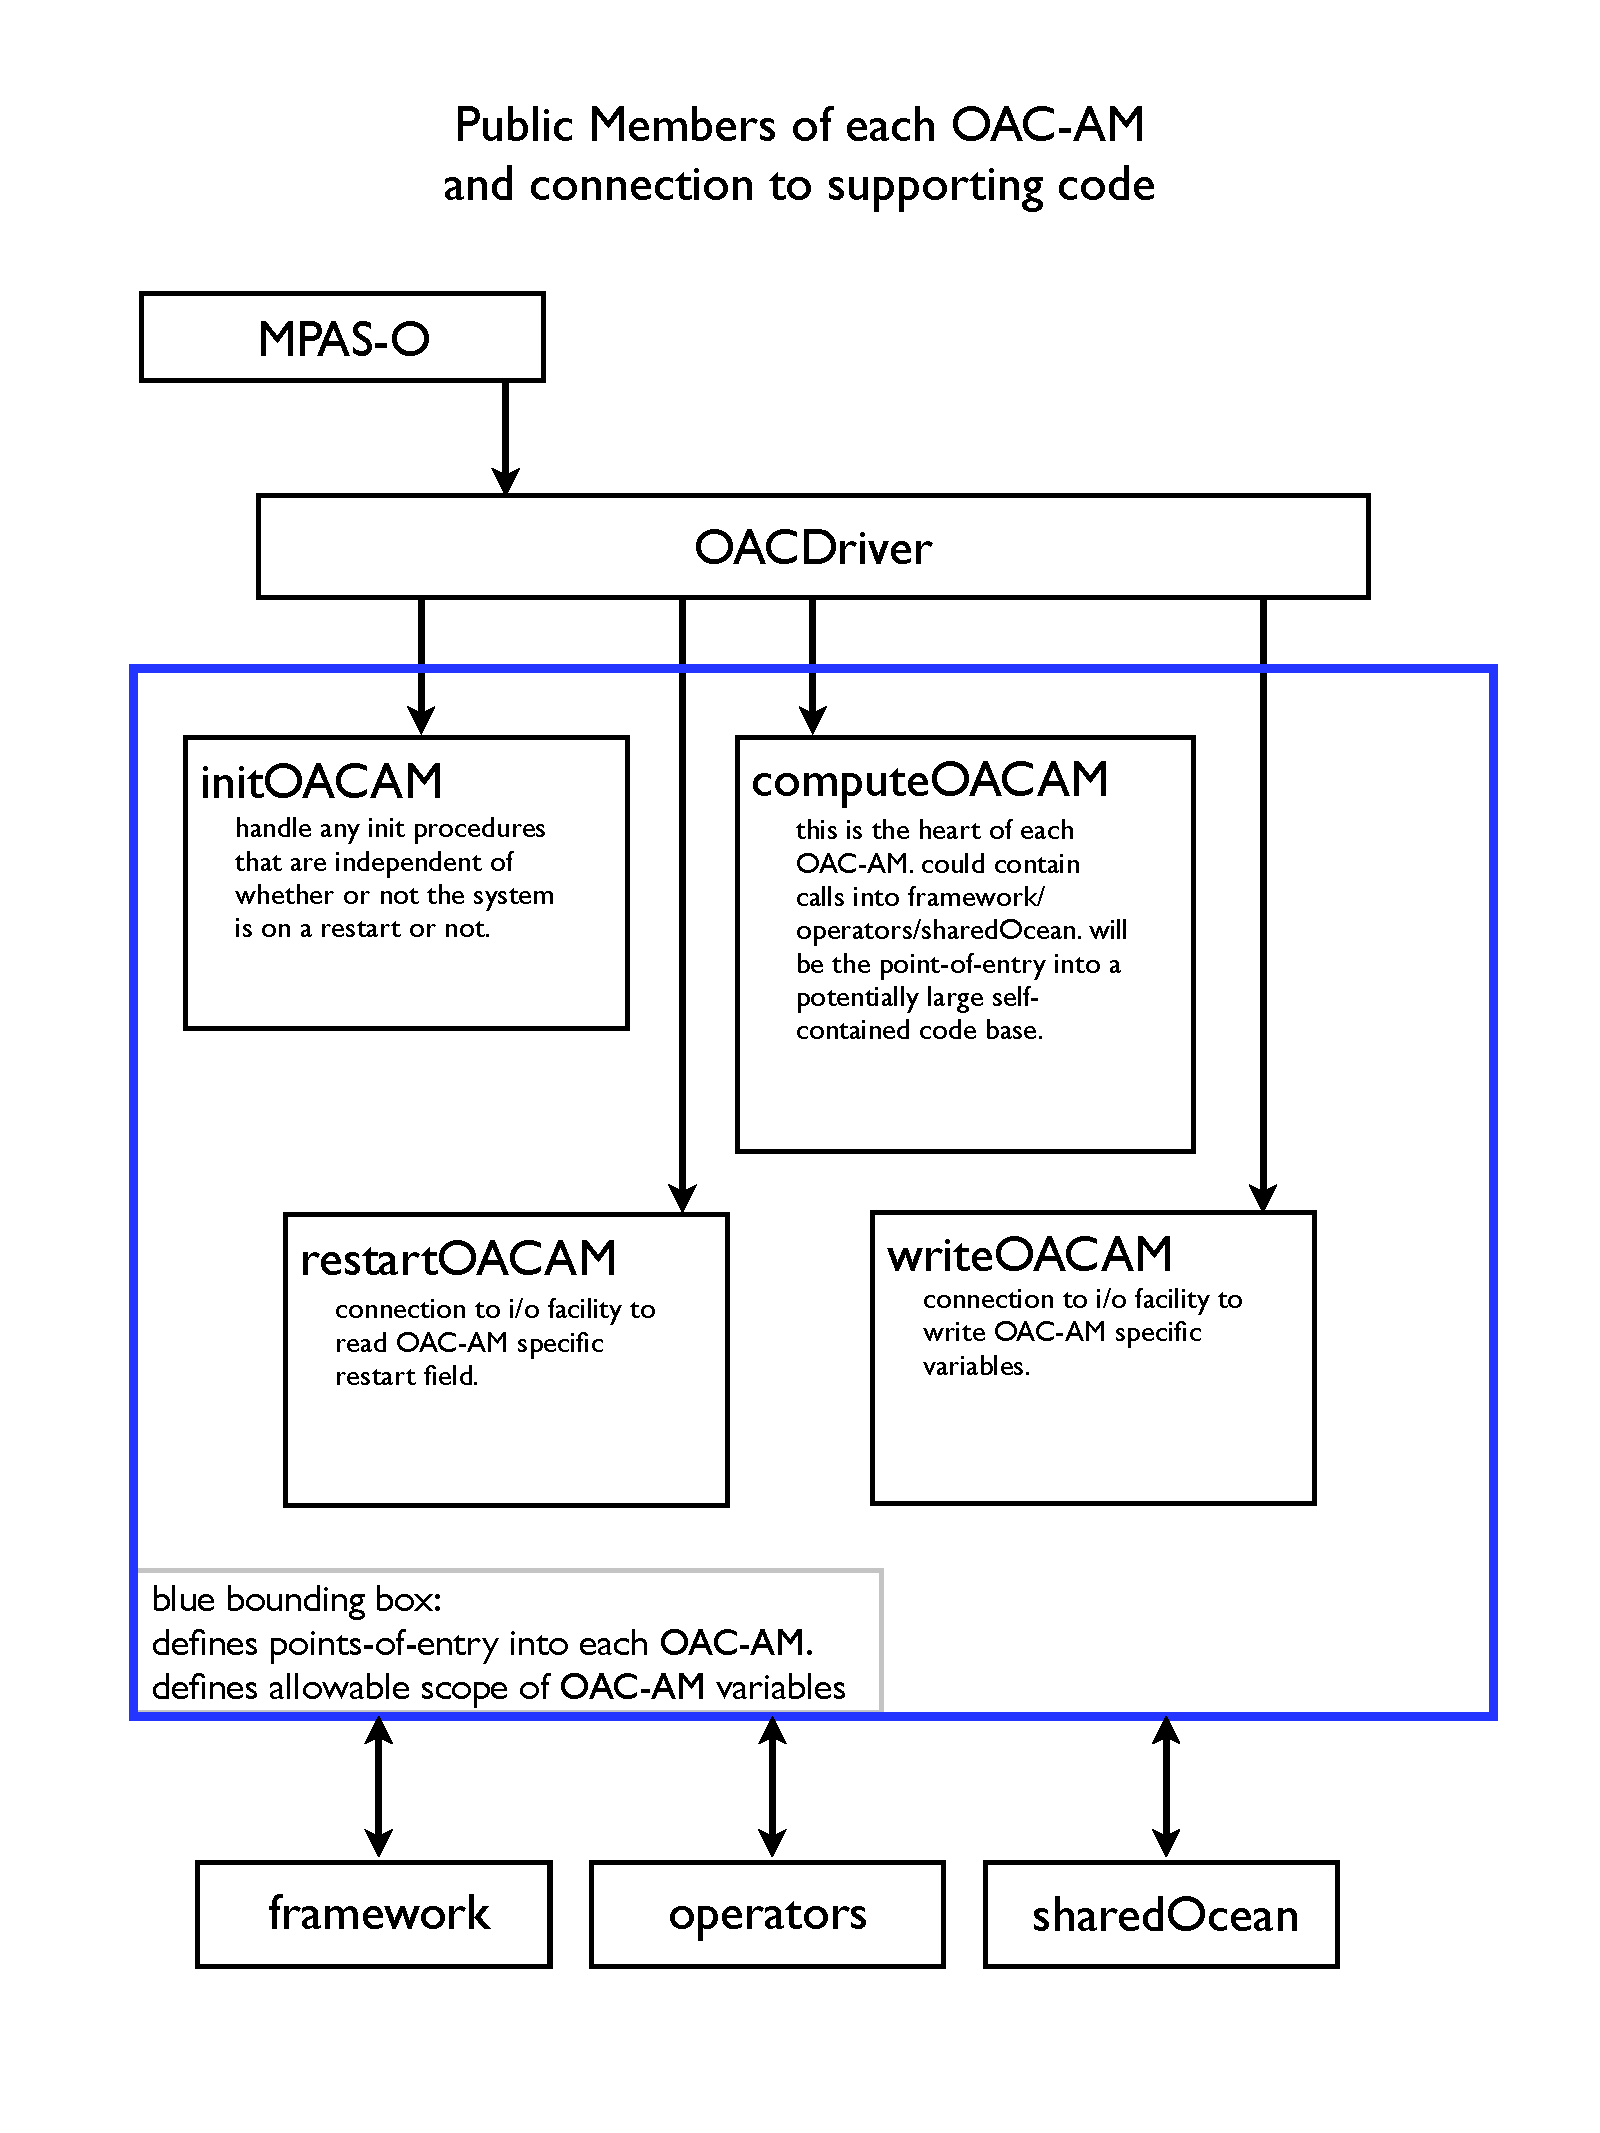
\includegraphics[width=12.0cm]{./figures/OAC-AM.pdf}} \\
\caption{Diagram outlining the calls into each analysis member.}
\label{OAC-AM}
\end{figure}

The new namelists for the ocean core will be:
\begin{verbatim}
&analysis
   config_write_analysis_on_startup = .true.
/
&am_name
   config_am_name_use = .true.
   config_am_name_file = "am_name.nc"
   config_am_name_interval = "0001_00:00:00"
/
&am_name2 etc.
\end{verbatim}
Additional flags may be added for each analysis member.
Until multiple output streams is available, only the following option will be supported
\begin{verbatim}
   config_am_name_file = "standard_output_file"
   config_am_name_interval = "standard_output_interval"
\end{verbatim}
which sets these values to be the same as config\_output\_name and config\_output\_interval in the io namelist.

The new namelists for the ocean analysis core will be:
\begin{verbatim}
&io
   config_file_name = "output.0000-01-01_00.00.00.nc"
   config_file_name_list = "file_name_list"
   config_first_record = 1
   config_record_interval = 1
   config_last_record = 1000
   config_pio_num_iotasks = 0
   config_pio_stride = 1
/
&am_name
   config_am_name_use = .true.
   config_am_name_file = "am_name.nc"
   config_am_name_interval = "0001_00:00:00"
/
&am_name2 etc.
\end{verbatim}
If \verb|config_file_name = "file"| then the analysis core proceeds through the list of filenames provided in 
\verb|config_file_name_list|.  For each analysis member, the flags in am\_name and the variables in the structure amName are identical.  To avoid typing these in multiple places, the registry files will be structured as follows:
\begin{itemize}
\item core\_ocean
\begin{itemize}
\item Registry.xml  
\end{itemize}
\item core\_ocean\_analysis
\begin{itemize}
\item Registry.xml  
\item Registry\_oac\_namelists.xml  
\item Registry\_oac\_variables.xml  
\end{itemize}
\end{itemize}
where flags and variables pertaining to an analysis member appear only once in Registry\_oac\_namelists.xml and  Registry\_oac\_variables.xml, respectively, and these files are inserted within Registry.xml at the beginning of the make process.



%-----------------------------------------------------------------------

\chapter{Testing}

After completion, a global simulation will be conducted with run-time analysis tools on.  Global diagnostics output will be compared between run-time, post-processed analysis core data, and global statistics from the current develop branch.  All three should match bit-for-bit on the same number of processors.  When processor counts vary, global statistics may not match in last digits due to order of operations.



%-----------------------------------------------------------------------

\end{document}
